% !TEX encoding = UTF-8 Unicode

\documentclass[twocolumn,10pt,a4j]{jsarticle}
\usepackage{kougai}
\usepackage{comment}
\usepackage{url}
\usepackage{graphics}


\title{ピアノ指導者の補助システムの提案}
\author{1532148 増田 彩美  指導教員 須田 宇宙 准教授}
\date{}

\begin{document}

\maketitle

\section{はじめに}

%背景
音楽は老若男女問わず,多くの人々を魅了するものである.
趣味として楽器演奏を挙げる人も多いことから,楽器と音楽が広く世界の人々に愛されるものであることがわかる.
日本ではピアノの奏者が200万人ほどいると言われている[1].大人から子どもまで様々な人がピアノを弾いているが,年代別に分類した場合多くは子どもがその割合を占める[2].それに従って個人から大手まで多くのピアノ教室が存在している.

%問題点
初心者にとってピアノの楽譜は難易度が高く,最初に楽譜が読めないことで挫折する人が多いという問題が存在する.そこで,教室では各音符に手書きでピアノの音階を書き込む工夫がなされている.しかし,それが指導者にとって負担になってしまっている現状がある.また,楽譜の上段と下段で拍子や音符の種類が異なる場合,どの音符を左右同時に弾くべきか分かりづらく,指導者が即座に判断することが難しい.

%目的
そこで本研究では,指導者を支援するシステムを制作し,その有用性を検証することを目的とする.


\section{ピアノの指導手順について}
ピアノを指導する手順は多くあり一概に形が決まっているわけではない.だが,どの手順でも最初に教える重要な部分は共通している.それは楽譜の基本的なルールを教えるということである.

しかし,前述したように,初心者にとってピアノを演奏しながら音階を一瞬で判断することは難しく,挫折の一因になりやすい.そこで,最初は音階の表示がある楽譜を用い演奏をする.そして,それと同時に楽譜を読む練習をし,やがて音階を表示しなくても弾けるようになるのが一般的な流れである.

そのため指導者は音階が書かれている楽譜を用意するか,自身で音階を書きこまなければならず,コストがかかる.そこで容易に楽譜をデータ化し,自動で音階表記をつけることができるシステムを制作することで,より指導の効率化や,汎用性の向上が見込めると考える.

\section{システムの概要}

\begin{figure}[h]
\begin{center}
 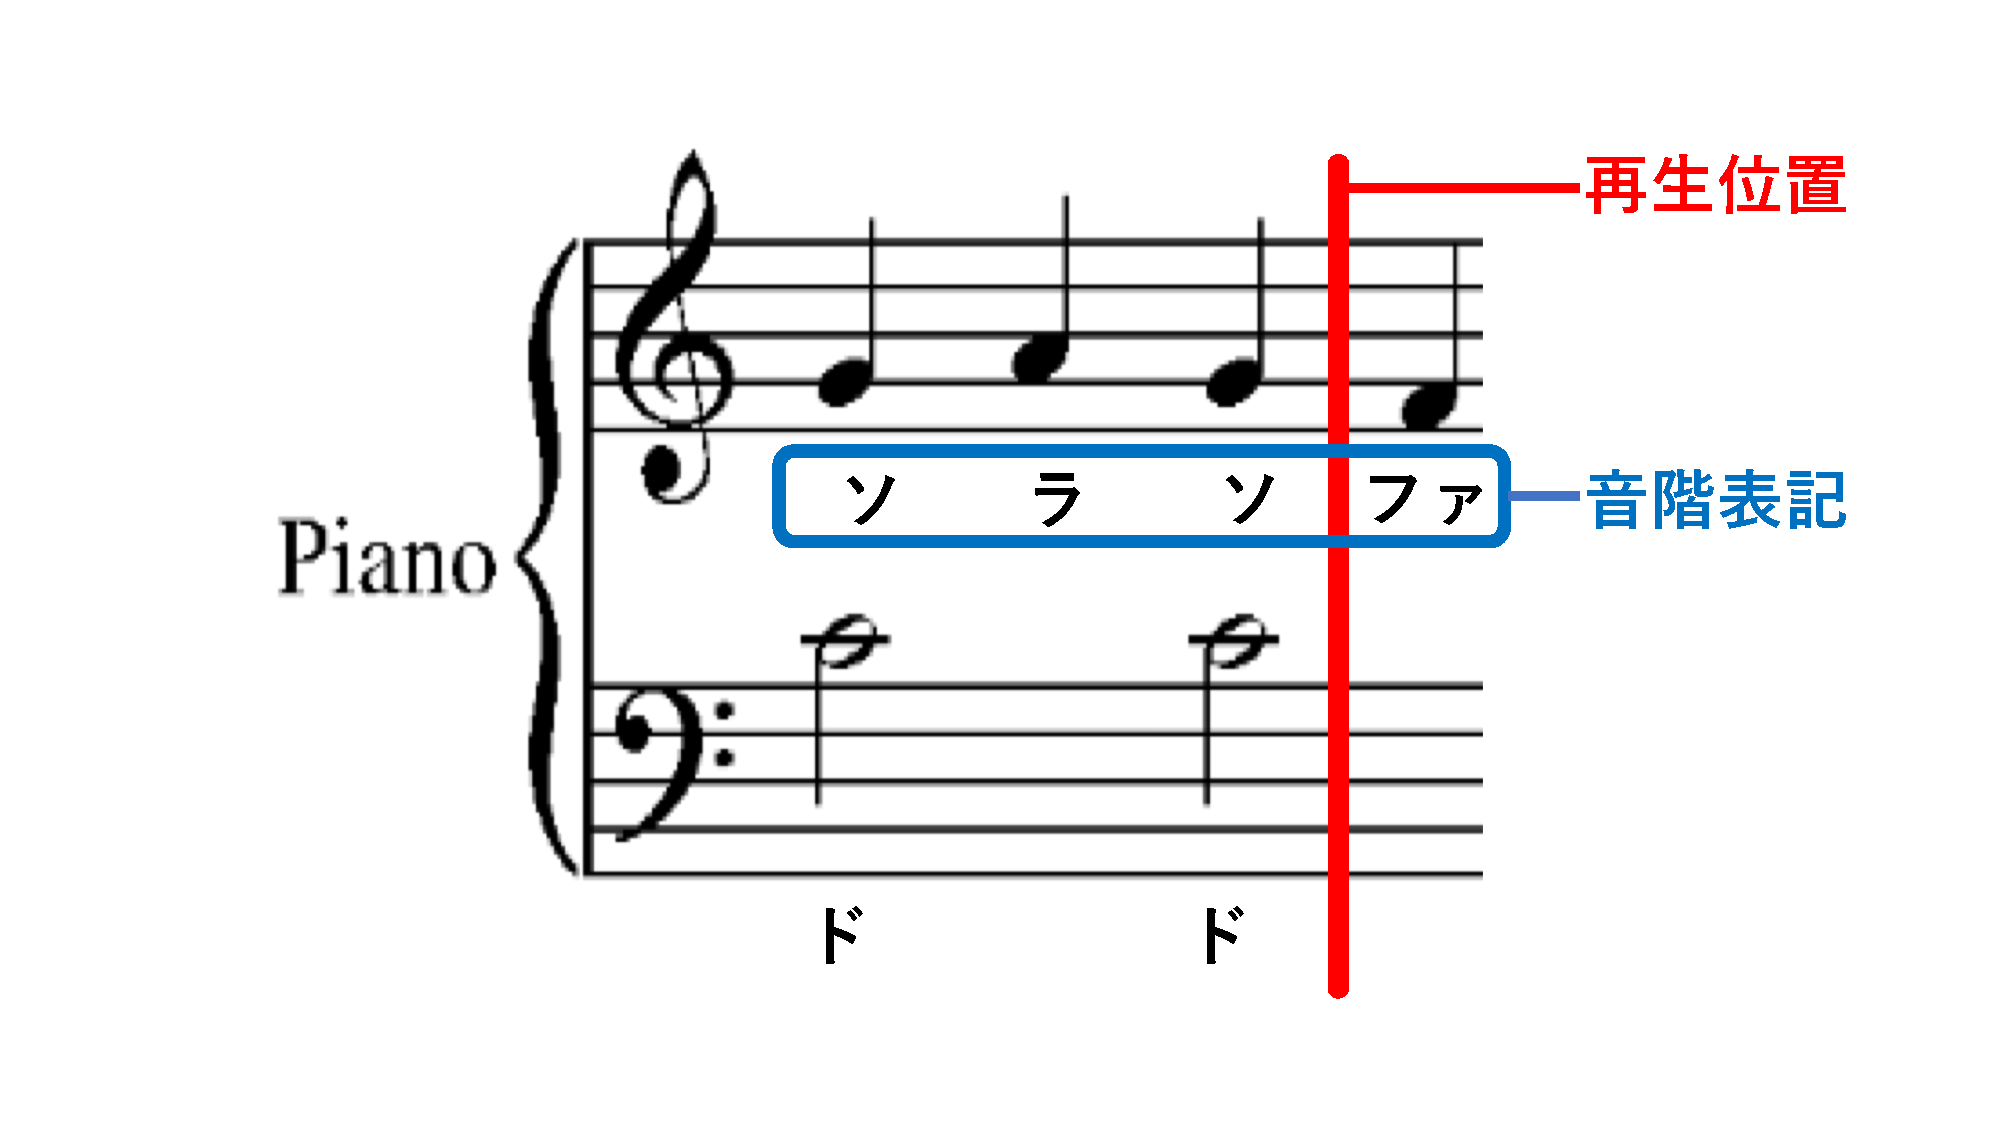
\includegraphics[clip,width=85mm,height=55mm]{image2.pdf}
\end{center}
 \caption{指導者支援システム概要}
 \label{fig:教科書}
\end{figure}
本研究ではピアノ指導者を補助するシステムを制作する.楽譜を写真で撮影し,2値化処理傾き補正などを施し楽譜をPDF化する.それをPythonのOpenCVにより解析し,音階の表記をつけることで各音符に音階を付与させる.また,楽譜に赤い線を表示することで同時に弾くべき音をわかりやすく表示する.Pythonで分析した各音符にMIDIで音情報を加えることで視覚だけではなく,聴覚のサポートも行う.実際に作成するシステムの画面概要を図1で表す.

また,これ以外にもいくつか機能を実装する予定である.
機能一覧を以下に示す.

\begin{enumerate}
%\renewcommand {\labelenumi}{(\arabic{enumi})}
\item 楽譜のPDF化
\item 各音符の音階表記
\item 線による演奏箇所表示
\item MIDIによる楽曲再生
\item 変化記号のある音符表記
\end{enumerate}

楽譜によって音符に変化記号がついているものがある.変化記号とは,シャープ(♯)やフラット(♭)といった,音を半音単位で高くしたり低くするための記号である.初心者にとって変化記号は見逃してしまうことが多い.そのため,変化記号がついている音階をわかりやすく表記する機能を実装する.

\section{今後の予定}
実際にシステムを制作し,それをピアノ指導者に評価してもらうことで有用性の検証を行う.

\begin{thebibliography}{99}
\bibitem{suda2018} 総務省: ``平成28年社会生活基本調査-生活行動に関する結果-'', \url{http://www.stat.go.jp/data/shakai/2016/pdf/gaiyou.pdf}, (参照 2018-8-23)

\bibitem{suda2018} 政府統計の総合窓口 e-Stat: ``「社会生活基本調査」における「趣味娯楽=楽器演奏」の行動者率(全国集計)'', \url{https://www.e-stat.go.jp/dbview?sid=0003192947}, (参照 2018-8-23)

\bibitem{suda2018}板東慶一郎:``楽譜認識を活用した演奏支援ソフトウェア'',\url{https://waseda.repo.nii.ac.jp/index.php?action=pages_view_main&active_action=repository_action_common_download&item_id=17358&item_no=1&attribute_id=20&file_no=1&page_id=13&block_id=21}, (参照 2018-8-23)

\end{thebibliography}


\end{document}